% Unofficial University of Cambridge Poster Template
% https://github.com/andiac/gemini-cam
% a fork of https://github.com/anishathalye/gemini
% also refer to https://github.com/k4rtik/uchicago-poster

\documentclass[final]{beamer}

% ====================
% Packages
% ====================

\usepackage[T1]{fontenc}
\usepackage{lmodern}
\usepackage[orientation=portrait,size=a1,scale=1.15]{beamerposter}
\usetheme{gemini}
\usecolortheme{nott}
\usepackage{graphicx}
\usepackage{booktabs}
\usepackage{tikz}
\usepackage{pgfplots}
\pgfplotsset{compat=1.14}
\usepackage{anyfontsize}

% ====================
% Lengths
% ====================

% If you have N columns, choose \sepwidth and \colwidth such that
% (N+1)*\sepwidth + N*\colwidth = \paperwidth
\newlength{\sepwidth}
\newlength{\colwidth}
% \setlength{\sepwidth}{0.025\paperwidth}
% \setlength{\colwidth}{0.45\paperwidth}
\setlength{\sepwidth}{0.025\paperwidth}
\setlength{\colwidth}{0.3\paperwidth}

\newcommand{\separatorcolumn}{\begin{column}{\sepwidth}\end{column}}

% ====================
% Title
% ====================

\title{x86 Architecture}

\author{William Bland}

% ====================
% Footer
% ====================

% \footercontent{
%   % \href{https://github.com/TheBlandit/EMC-x86}{https://github.com/TheBlandit/EMC-x86} \hfill
%   % \href{https://exetermathematicsschool.ac.uk/}{Exeter Mathematics School}
% }

% ====================
% Logo
% ====================

\logoright{
\includegraphics[height=3.5cm]{logos/ems_logo.png}\hspace{20ex}}
% \logoleft{\hspace{20ex}
\includegraphics[height=3.0cm]{logos/x86.png}}

% ====================
% Body
% ====================

\begin{document}

% Refer to https://github.com/k4rtik/uchicago-poster
% logo: https://www.cam.ac.uk/brand-resources/about-the-logo/logo-downloads
% \addtobeamertemplate{headline}{}
% {
%     \begin{tikzpicture}[remember picture,overlay]
%       \node [anchor=north west, inner sep=3cm] at ([xshift=-2.5cm,yshift=1.75cm]current page.north west)
%       {\includegraphics[height=7cm]{logos/unott-logo.eps}}; 
%     \end{tikzpicture}
% }

\begin{frame}[t]
\begin{columns}[t]
\separatorcolumn

\begin{column}{\colwidth}
  \begin{block}{Overview of the x86 architecture}
    Every processor contains an architecture which describes how it executes machine code.
    A common architecture for desktop processors to use is x86, this means that the same programs can be run across different x86 processors without the need to be rewritten.

    Below is a brief history of x86 processors, summarising the major changes.
    \begin{itemize}
      \item The first x86 processor was the x8086 and was 16-bit, it used memory segmentation to allow it to separate the address space for processes, and to give it access to 1MiB of memory
      \item The i286 introduced memory protection which changed the segmentation model to prevent processes from accessing memory they did not own
      \item The i386 was the first 32-bit processor, introducing 32-bit registers and paging (which is another form of memory management in addition to segmentation)
      \item The i486 introduced an integrated x87 FPU (previously they were a separate processor)
      \item The intel Pentium 4 introduced 64-bit extensions
    \end{itemize}
  \end{block}

  \begin{block}{Memory Management}
    The kernel has to manage the usage of memory that processes use (give memory to programs that request it, and to prevent a program accessing the memory of another).

    In real mode, memory segmentation is used.
    When accessing memory, the value in the segment register is multiplied by 16 and added to the effective address, which produces the physical address of the memory.
    This allows a program to be split into logical sections (one for each segment register), allows access to 1MiB of memory (due to a 20-bit address bus), and the memory used by different processes are kept separate by keeping them in different segments.
    However it does not prevent a program from accessing memory it has not been allocated, and is difficult to manage memory spanning multiple segments.

    \begin{figure}[H]
        \centering
        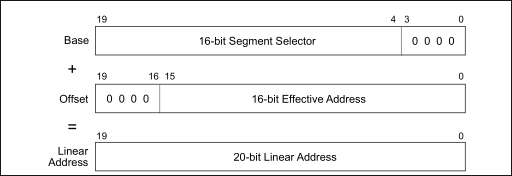
\includegraphics[width=0.5\textwidth]{./pictures/real_address.png}
        \caption{Real mode address translation}
    \end{figure}

    In protected mode, memory protection is enabled; this modifies the segmentation method so the segment registers are now segment selectors into a kernel-defined segment descriptor table.
    A segment descriptor contains the base address, limit (length of the segment), and flags (permissions) of the segment which provides greater flexibility of the use of memory segments.
    Unlike real mode, this prevents processes accessing memory they have not been allocated, however it still requires programs to manage their use of segments.
    Furthermore, segmentation allows for the use of different models, below are diagrams of a few common models.

    \begin{figure}[!htb]
    \minipage{0.32\textwidth}
      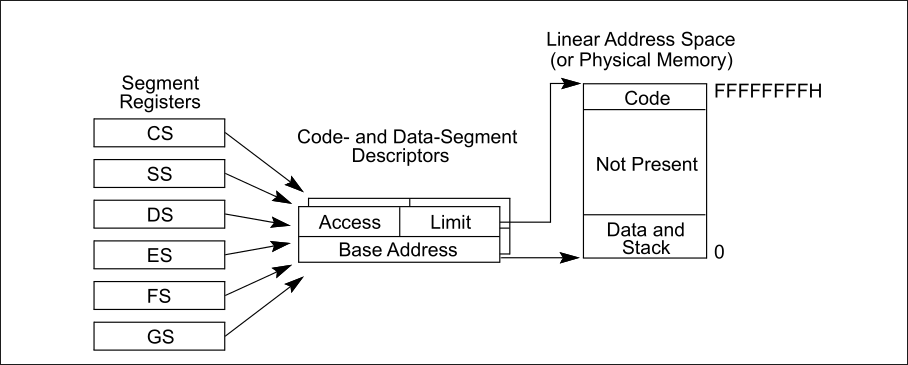
\includegraphics[width=\linewidth]{./pictures/flat.png}
      \caption{Flat (simple, no protection)}
    \endminipage\hfill
    \minipage{0.32\textwidth}
      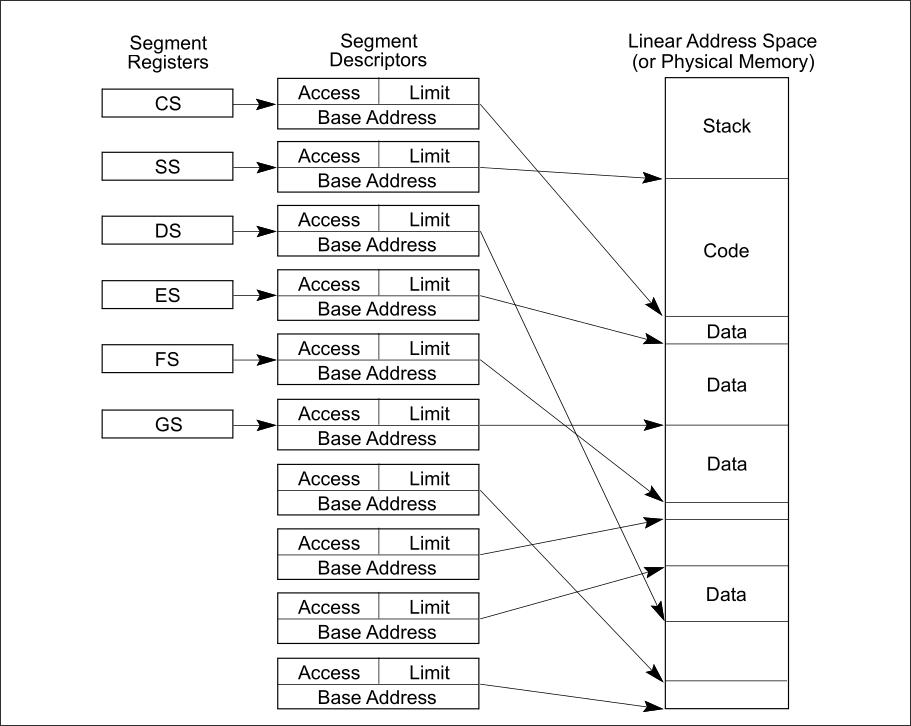
\includegraphics[width=\linewidth]{./pictures/multi_segment.png}
      \caption{Multi-segment (complex, full use of segmentation)}
    \endminipage\hfill
    \minipage{0.32\textwidth}
      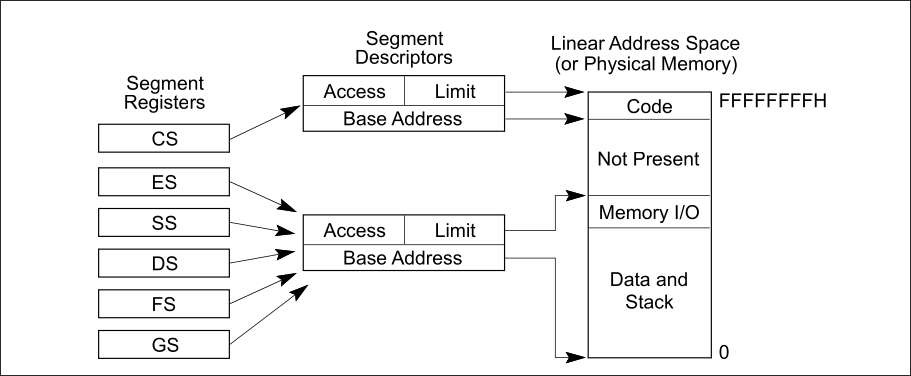
\includegraphics[width=\linewidth]{./pictures/protected_flat.png}
      \caption{Protected Flat (simple, protection against invalid addresses)}
    \endminipage
    \end{figure}

    Paging splits up the address space into 4KiB pages, and introduces the paging hierarchy which is a memory structure that the kernel manages and the hardware automatically traverses to convert a linear address into a physical address.
    This method provides greater control than segmentation by controlling the abilities of specific pages, and is completely transparent to the program (so is easier to use than segmentation (which requires keeping track of segment selectors)).
    Furthermore paging allows contiguous linear addresses to use non-contiguous physical address, which prevents external memory fragmentation and makes it easier for programs to allocate/free memory.

    \begin{figure}[H]
      \centering
      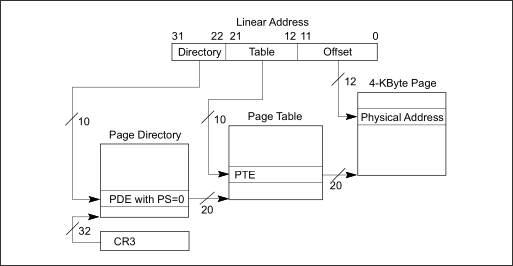
\includegraphics[width=0.5\textwidth]{./pictures/paging.png}
      \caption{Translation of linear to physical address using 32-bit paging (other paging methods use additional layers)}
    \end{figure}
  \end{block}
\end{column}

\separatorcolumn

\begin{column}{\colwidth}
  \begin{block}{Operating modes}
    x86 processors have several operating modes which change how machine code is executed.

    \begin{itemize}
      \item Real: \\
        All x86 processors start in real address mode at address FFFF:0000.
      \item Protected: \\
        Enables memory protection, enables the use of paging and a 32-bit instruction set, allowing the use of a larger address space and more multitasking features.
      \item Long mode: \\
        Enables the use of 64-bit registers and instructions, allowing a larger address space.
        Furthermore it runs in two sub modes, one for 64-bit code and one for 32-bit compatibility mode.
    \end{itemize}
  \end{block}

  \begin{block}{Caching}
    Processors contain cache (which stores recently read/written data) to prevent having to access main memory (which is much slower than accessing cache).
    Cache is split up into cache lines, and x86 uses the MESI cache coherency protocol to keep the cache lines in different processors valid.
    Each cache line has a MESI state, writes/reads to the cache line from the current processor/other processors affect the MESI state.

    \begin{figure}[H]
        \centering
        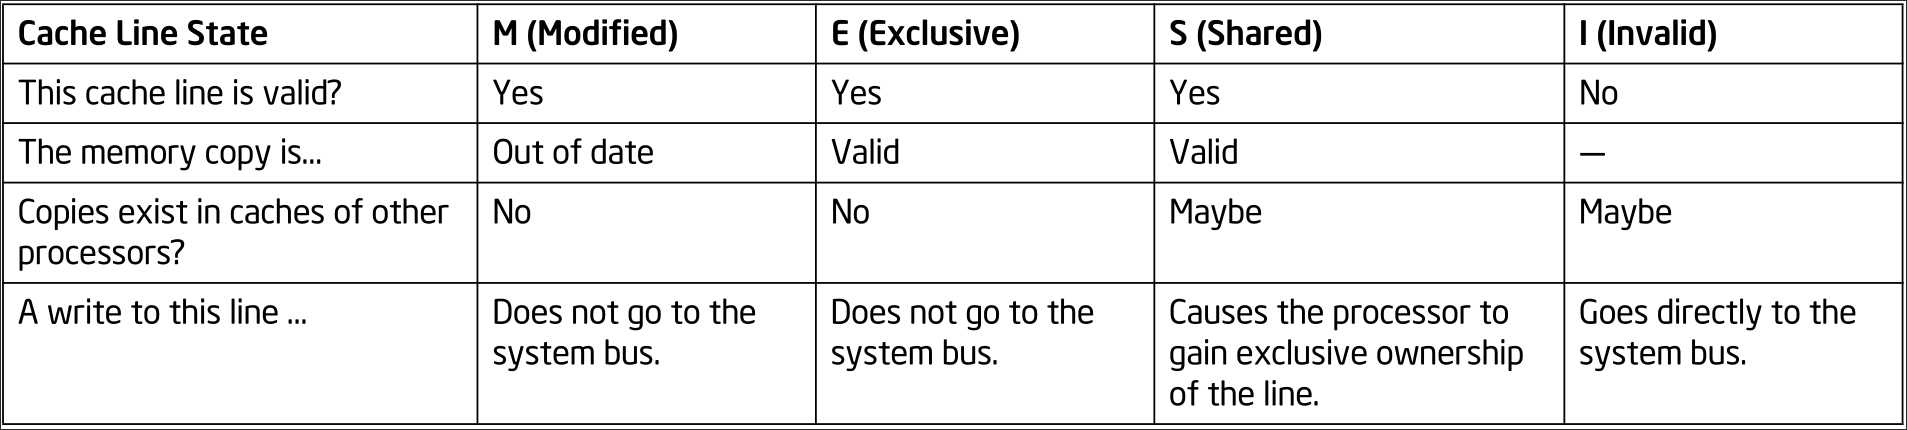
\includegraphics[width=\textwidth]{./pictures/mesi.png}
        \caption{MESI states}
    \end{figure}

    Before writing to cache, the processor pushes writes to a store buffer, this means that a write may not be immediately globally visible, a memory fence or LOCK prefix can be used to flush the store buffer (which updates all the cache states).

    Furthermore there is another cache called the TLB (Translation Lookaside Buffer) which stores recent translations of the linear to physical address translation due to paging (which prevents unnecessary hardware assisted page walks).
    When updating a page table, the kernel must invalidate the TLB entries which contain the invalid page entries. 
  \end{block}

  \begin{block}{Registers}
    The processor contains many registers which can be directly accessed using instructions.
    One type of register are general purpose registers which can be used by most instructions and so can be used for most operations, these registers are split up into multiple registers, for example the 32-bit EAX register is located in the lower 32 bits of the 64-bit RAX register.
    Control registers control the operation of the processor, for example CR3 contains the base address of the paging hierarchy.
    Segment registers are used in segmentation and are always 16-bit.
    Model Specific Registers (MSRs) are only present on some processors and are accessed with specific instructions, one use of them is used to enable long mode extensions.

    \begin{figure}[H]
        \centering
        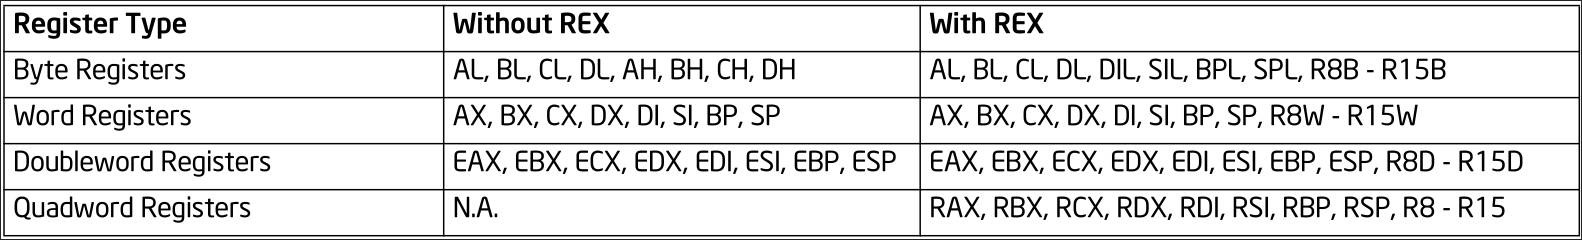
\includegraphics[width=\textwidth]{./pictures/rex_registers.png}
        \caption{General purpose registers available to x86 instructions (see Instructions for details on REX)}
    \end{figure}
  \end{block}

  \begin{block}{Interrupts}
    Occasionally a hardware device will require immediate attention or an instruction could have raised an exception, this will require the current process to be interrupted and run code to handle the interrupt (which is called an Interrupt Service Routine (ISR)).
    Interrupt descriptors contain information on how the interrupt should be handled and are stored inside an interrupt descriptor table which its address is stored within the Interrupt Descriptor Table Register.
    Since an interrupt is able to occur during the execution of a program, the ISR must restore the state of the processor to the state it was in when the interrupt occurred;
    whilst the instruction \texttt{iret} (interrupt return) is able to restore registers such as RIP and RFLAGS, the ISR must restore any registers it modified (eg general purpose registers).
  \end{block}
\end{column}

\separatorcolumn

\begin{column}{\colwidth}
  \begin{block}{BIOS/UEFI}
    Most x86 processors are used within an IBM PC Compatible environment (a common environment which includes various hardware devices such as a PIC, and a BIOS).
    The BIOS (Basic Input/Output System) is firmware ran during processor start up which transfers control over to the operating system, it is used to perform hardware initialisation and can perform operations requested by the OS through BIOS interrupts.
    The BIOS supports a form of output called VGA text mode, it uses a region of memory as memory-mapped IO;
    this region of memory is treated as an array of 16-bit characters on the screen (the lower byte is the character and the higher byte is its attribute (eg colour)).

    The UEFI (Unified Extensible Firmware Interface) is a replacement for the legacy BIOS system.
    After the BIOS initialises hardware, it drops back into a backwards-compatible real mode, which means the bootloader must initialise the A20 gate, GDT, LDT, and switch to protected/long mode;
    UEFI performs these steps, simplifying the boot process.
    UEFI contains many standardised functions which can be found through a system table and called by the OS, in comparison to BIOS interrupts which are not standardised.
    The UEFI bootloader contains entries which consist of a drive partition and a path, the drive partition points to the EFI System Partition (ESP, usually FAT32), and the path points to the EFI bootloader file in the partition.
  \end{block}

  \begin{block}{Syscalls (Linux)}
    Syscalls are a type of interrupt which allows user code to request resources from the kernel.
    32-bit code uses the interrupt \texttt{int 80h} whilst 64-bit code uses the instruction \texttt{syscall}.
    Before calling a syscall, the user code must place its arguments into specific registers.
    For example in a 64-bit \texttt{read} syscall (used for reading bytes from an open file descriptor) the syscall number 0 (for read) is placed in EAX, the file descriptor to be read from is placed in RDI, the pointer to the buffer (where the bytes will be written to) is placed in RSI, and the (max) number of bytes to be read is placed in RDX.
    When the syscall has completed its status is stored in RAX, for \texttt{read} a non-negative integer represents a success and the number of bytes actually read, and a negative integer represents an error that occurred.
  \end{block}

  \begin{block}{Instructions}
    The machine code that processors execute contains a list of instructions encoded in binary.
    There are various types of instruction that can be executed such as: arithmetic (mathematical operations eg \texttt{ADD}), logic (boolean logic eg \texttt{XOR}), memory (manipulating memory eg \texttt{MOV}), comparison (setting RFLAGS registers based on a comparison eg \texttt{CMP}), and control (moving execution to another part of the program eg \texttt{JMP}).

    When assembly code is translated to machine code, a program called an assembler (eg nasm) converts the assembly code into object code.
    An object code file may contain part of the machine code for a program, it also contains placeholder symbols and offsets (eg if the symbol existed in another file).
    Multiple object code files can be linked together using a program called a linker (eg ld) to create an executable file, this process resolves the placeholder symbols and offsets in the object files.

    Furthermore, the x86-64 bit extensions introduced the REX prefix;
    the REX prefix is able to promote the following instruction to use x86-64 extensions (eg access to additional registers and increase the operand size to 64 bits).
    Unlike the LOCK prefix, the REX prefix is automatically added by most assemblers.
  \end{block}

  \begin{block}{Multithreading}
    On multiprocessor (multithreaded) environments, race conditions can occur when two threads simultaneously access the same memory region, resulting in undefined behaviour.
    Race conditions can be prevented by using a mutex (provides a lock over a region of memory allowing for exclusive access to the region of memory for a single thread), however the locking of the mutex itself might be subject to race conditions.
    In order to overcome this, hardware synchronisation is required.
    The \texttt{LOCK} prefix can be used on specific instructions such as \texttt{CMPXCHG} to make them atomic, this means that the processor has exclusive access to the cache line being used;
    therefore the memory being used as the mutex lock can be read, compared and written without the risk of another thread accessing the value between the read and write, which prevents race conditions.
    Furthermore memory fences can be used to prevent issues caused by out-of-order execution by preventing loads/stores being reordered to occur after the fence.
  \end{block}
\end{column}
\separatorcolumn

\end{columns}
\end{frame}
\end{document}
